\documentclass{beamer}


\usepackage{amssymb,amsmath}
\usepackage{graphicx}
\usepackage{url}
\usepackage{color}
\usepackage{relsize}		% For \smaller
\usepackage{url}			% For \url
\usepackage{epstopdf}	% Included EPS files automatically converted to PDF to include with pdflatex
\usepackage{pagenote}[continuous,page]

%For MindMaps
% \usepackage{tikz}%
% \usetikzlibrary{mindmap,trees,arrows}%

%%% Color Definitions %%%%%%%%%%%%%%%%%%%%%%%%%%%%%%%%%%%%%%%%%%%%%%%%%%%%%%%%%
%\definecolor{bordercol}{RGB}{40,40,40}
%\definecolor{headercol1}{RGB}{186,215,230}
%\definecolor{headercol2}{RGB}{80,80,80}
%\definecolor{headerfontcol}{RGB}{0,0,0}
%\definecolor{boxcolor}{RGB}{186,215,230}

%%% Save space in lists. Use this after the opening of the list %%%%%%%%%%%%%%%%
%\newcommand{\compresslist}{
%	\setlength{\itemsep}{1pt}
%	\setlength{\parskip}{0pt}
%	\setlength{\parsep}{0pt}
%}

%\setbeameroption{show notes on top}

% You should run 'pdflatex' TWICE, because of TOC issues.

% Rename this file.  A common temptation for first-time slide makers
% is to name it something like ``my_talk.tex'' or
% ``john_doe_talk.tex'' or even ``discrete_math_seminar_talk.tex''.
% You really won't like any of these titles the second time you give a
% talk.  Try naming your tex file something more descriptive, like
% ``riemann_hypothesis_short_proof_talk.tex''.  Even better (in case
% you recycle 99% of a talk, but still want to change a little, and
% retain copies of each), how about
% ``riemann_hypothesis_short_proof_MIT-Colloquium.2000-01-01.tex''?

\mode<presentation>
{
  % A tip: pick a theme you like first, and THEN modify the color theme, and then add math content.
  % Warsaw is the theme selected by default in Beamer's installation sample files.

  %%%%%%%%%%%%%%%%%%%%%%%%%%%% THEME
  %\usetheme{Madrid}		% No subsection
  \usetheme{AnnArbor}  % Subsection on top, no color


  %\usetheme{Antibes}
  %\usetheme{Bergen}
  %\usetheme{Berkeley}		% bem bacana - menu esquerdo
  %\usetheme{Berlin}
  %\usetheme{Boadilla}
  %\usetheme{boxes}
  %\usetheme{CambridgeUS}		% bem bacana - menu superior
  %\usetheme{Copenhagen}
  %\usetheme{Darmstadt}
  %\usetheme{default}
  %\usetheme{Dresden}
  %\usetheme{Frankfurt}
  %\usetheme{Goettingen}
  %\usetheme{Hannover}		% bem bacana - menu esquerdo
  %\usetheme{Ilmenau}
  %\usetheme{JuanLesPins}
  %\usetheme{Luebeck}
  %\usetheme{Malmoe}
  %\usetheme{Marburg}		% bem bacana - menu direito
  %\usetheme{Montpellier}
  %\usetheme{PaloAlto}		% bem bacana - menu esquerdo
  %\usetheme{Pittsburgh}
  %\usetheme{Rochester}		%bacana
  %\usetheme{Singapore}
  %\usetheme{Szeged}
  %\usetheme{Warsaw}

  %%%%%%%%%%%%%%%%%%%%%%%%%%%% COLOR THEME
  %\usecolortheme{default}		% branco, azul clarinho
  \usecolortheme{crane}		% Very yellow (ok)

  %\usecolortheme{albatross}		% azul escuro, massa
  %\usecolortheme{beetle}		% cinza, menu azul
  %\usecolortheme{dolphin}		% azul e branco, legal
  %\usecolortheme{dove}			% cinza e branco, feio
  %\usecolortheme{fly}			% todo cinza, horrível
  %\usecolortheme{lily}			% parece o default
  %\usecolortheme{orchid}		% azul e branco, ok
  %\usecolortheme{rose}			% branco e violeta-claro, bonito
  %\usecolortheme{seagull}		% cinza, feio
  %\usecolortheme{seahorse}		% nhé, meio feio
  %\usecolortheme{sidebartab}		% Azul, branco, destaque na tab, interessante
  %\usecolortheme{structure}		% bichado
  %\usecolortheme{whale}		% Azul e branco, bem bonito

  %%%%%%%%%%%%%%%%%%%%%%%%%%%% OUTER THEME
  \useoutertheme{default}
  %\useoutertheme{infolines}
  %\useoutertheme{miniframes}
  %\useoutertheme{shadow}
  %\useoutertheme{sidebar}
  %\useoutertheme{smoothbars}
  %\useoutertheme{smoothtree}
  %\useoutertheme{split}
  %\useoutertheme{tree}

  %%%%%%%%%%%%%%%%%%%%%%%%%%%% INNER THEME
  \useinnertheme{circles}
  %\useinnertheme{default}
  %\useinnertheme{inmargin}
  %\useinnertheme{rectangles}
  %\useinnertheme{rounded}

  %%%%%%%%%%%%%%%%%%%%%%%%%%%%%%%%%%%

  \setbeamercovered{invisible} % or whatever (possibly just delete it)
  % To change behavior of \uncover from graying out to totally
  % invisible, can change \setbeamercovered to invisible instead of
  % transparent. apparently there are also 'dynamic' modes that make
  % the amount of graying depend on how long it'll take until the
  % thing is uncovered.

}


% Get rid of nav bar
\beamertemplatenavigationsymbolsempty

% Use short top
%\usepackage[headheight=12pt,footheight=12pt]{beamerthemeboxes}
%\addheadboxtemplate{\color{black}}{
%\hskip0.5cm
%\color{white}
%\insertshortauthor \ \ \ \
%\insertframenumber \ \ \ \ \ \ \
%\insertsection \ \ \ \ \ \ \ \ \ \ \ \ \ \ \ \ \  \insertsubsection
%\hskip0.5cm}
%\addheadboxtemplate{\color{black}}{
%\color{white}
%\ \ \ \
%\insertsection
%}
%\addheadboxtemplate{\color{black}}{
%\color{white}
%\ \ \ \
%\insertsubsection
%}

% Insert frame number at bottom of the page.
% \usefoottemplate{\hfil\tiny{\color{black!90}\insertframenumber}}

%% makes the ppagenote command for figure references at the end.

\usepackage[english]{babel}
%qq\usepackage[latin1]{inputenc}
\usepackage{CJKutf8}
\usepackage{subfigure}

\usepackage{times}
\usepackage[T1]{fontenc}

\makepagenote
\renewcommand{\notenumintext}[1]{}
\newcommand{\ppagenote}[1]{\pagenote[Page \insertframenumber]{#1}}

\title[Programming Challenges]{GB20602 - Programming Challenges}
\author[Claus Aranha]{Claus Aranha\\{\footnotesize caranha@cs.tsukuba.ac.jp}}
\institute[U. Tsukuba]{University of Tsukuba, Department of Computer Sciences}


\title[]{Software Science Seminar}
\subtitle[]{Week 7 - Graph Search}
\author[Claus Aranha]{Claus Aranha\\{\footnotesize caranha\@@cs.tsukuba.ac.jp}}
\institute{College of Information Sciences}
\date{2015-06-08\\{\tiny Last updatet \today}}

\begin{document}

\section{Introduction}
\subsection{Introduction}

\begin{frame}
\maketitle
\end{frame}


\begin{frame}
  \frametitle{Weeks 7 and 8}
  \begin{block}{Chapter 7 -- Graph Transversal}
    \begin{itemize}
    \item Characteristics;
    \item Representation;
    \item Transversal;
    \end{itemize}
  \end{block}
  \begin{block}{Chapter 8 -- Graph Algorithms}
    \begin{itemize}
    \item Network Flow;
    \item Bipartite Graphs;
    \item Spanning Trees;
    \end{itemize}
  \end{block}
\end{frame}

\begin{frame}
  \frametitle{Graphs Everywhere!}
  \begin{block}{}
    Graphs are one of the unifying themes of computer sciences: Many
    theoretical and application problems can be described or thought
    of as some sort of graph.
  \end{block}
  {\small
  \begin{columns}[c]
    \column{0.5\textwidth}
    \begin{itemize}
    \item Communication Networks
    \item Decision Trees
    \item Program Execution
    \item Human Relationships
    \item Geometric shapes
    \item Language Grammar
    \end{itemize}
    \column{0.5\textwidth}
    \begin{itemize}
    \item Transportation Networks
    \item Scheduling Restrictions
    \item Module Dependencies
    \item File System Structure
    \item Recurrence Relations
    \item Finite State Automata
    \end{itemize}
  \end{columns}}
\end{frame}

\begin{frame}
  \frametitle{Graph Examples: Network Graph}
  \begin{center}
    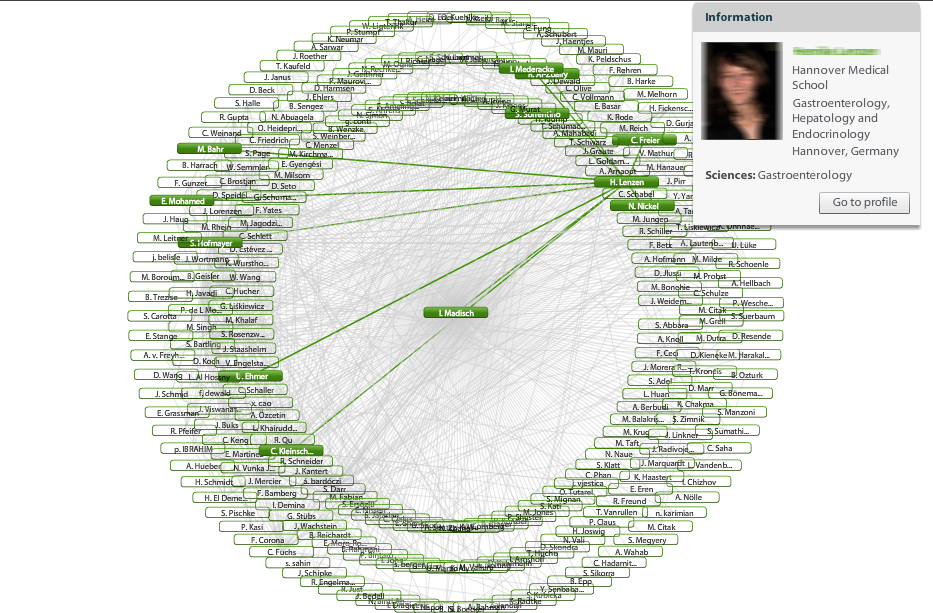
\includegraphics[width=0.7\textwidth]{img/networkgraph}
  \end{center}  
  \begin{block}{}
    {\small
    A Network Graph can represent the connections between people in a
    network. It shows how a minority of people are central nodes that
    connect many, while the majority only have a few connections.}
  \end{block}
  \hfill\tiny{Image from researchgate.net}
\end{frame}

\begin{frame}
  \frametitle{Graph Examples: Dependency Graph}
  \begin{center}
    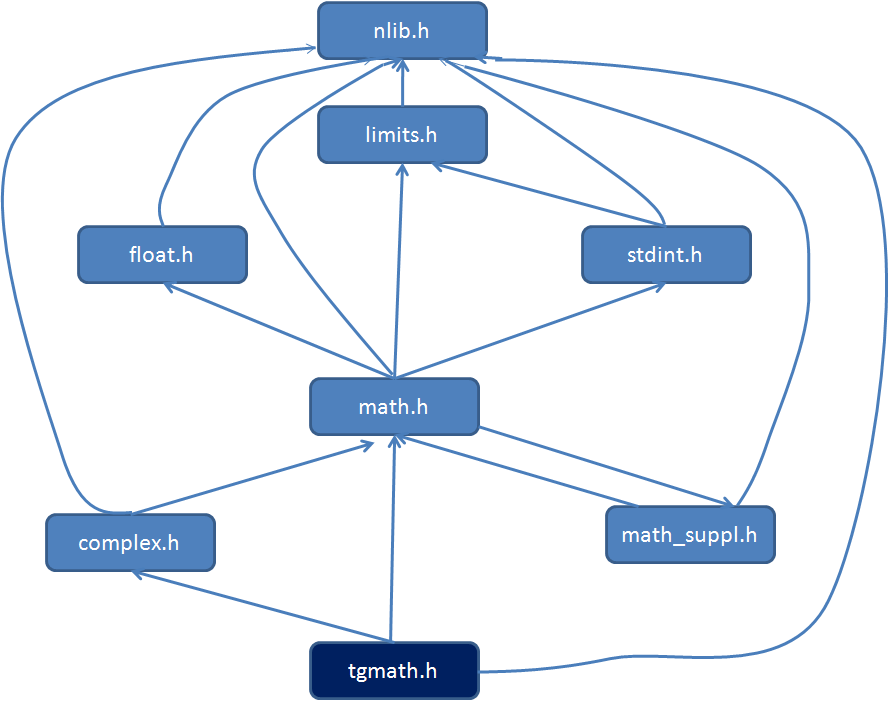
\includegraphics[width=0.6\textwidth]{img/dependencygraph}
  \end{center}  
  \begin{block}{}
    {\small A Dependency Graph links libraries and software packages by their
    direct dependencies. It can detect circular dependencies, or
    orphaned packages.}
  \end{block}
  \hfill\tiny{Image from Wikipedia}
\end{frame}

\begin{frame}
  \frametitle{Graph Examples: State Graph}
  \begin{center}
    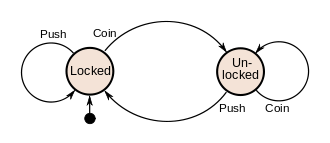
\includegraphics[width=0.8\textwidth]{img/stategraph}
  \end{center}  
  \begin{block}{}
    {\small The usual way to represent State machines is a state graph. You
    can see at a glance all the states and transitions of the state
    machine, and have an idea of what it does.}
  \end{block}
  \hfill\tiny{Image from Wikipedia}
\end{frame}

\begin{frame}
  \frametitle{Graph Examples: Grammar Graph}
  \begin{center}
    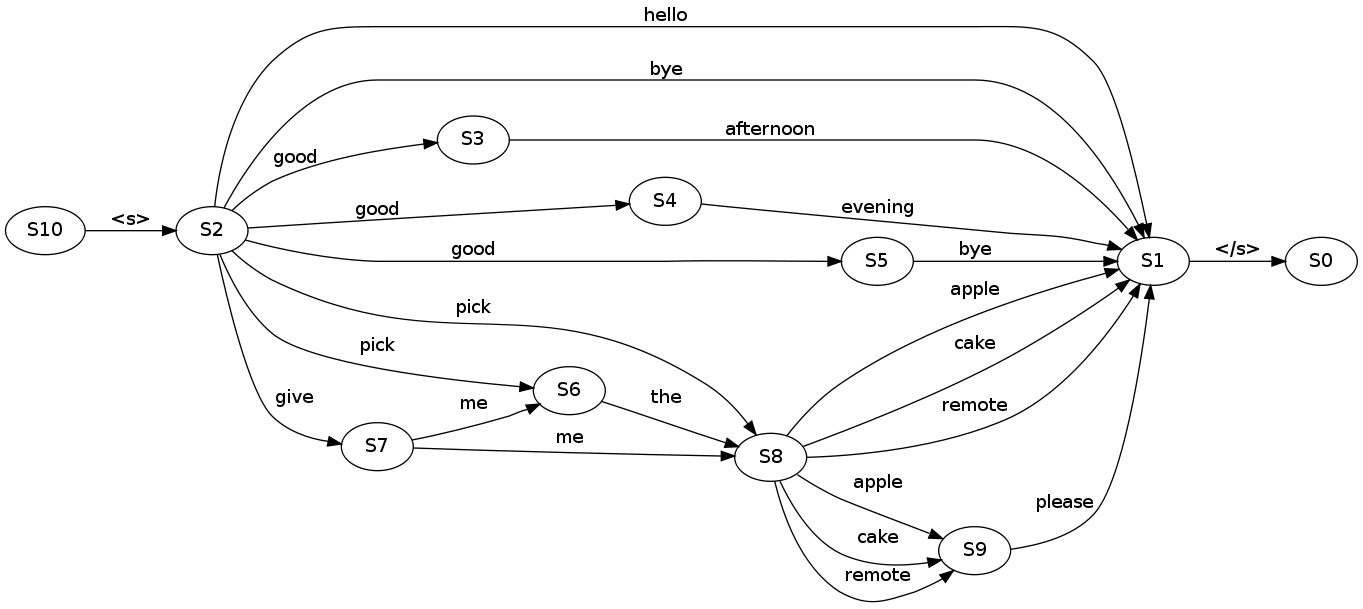
\includegraphics[width=0.8\textwidth]{img/grammargraph}
  \end{center}  
  \begin{block}{}
    {\small Gramma graphs show all possible sentences that can be generated
    from a given grammar. You can generate any sequences by walking
    the graph using different patterns.}
  \end{block}
  \hfill\tiny{Image from openhri.net}
\end{frame}



\section{Basic Characteristics}
\subsection{Definitions}

\begin{frame}
  \frametitle{Basic Definition}
  \begin{block}{Definition}
    \begin{itemize}
    \item A Graph $G=(V,E)$ is defined by a set $V$ of
      \structure{Vertices}, and a set $E$ of \structure{Edges}.
    \item An edge consists of an ordered or unordered pair of vertices
      from $V$.
    \end{itemize}
  \end{block}
  \begin{block}{}
    Graphs can be described by their properties, which influence how
    they can be represented and analyzed.
  \end{block}
\end{frame}

\begin{frame}
  \frametitle{Undirected x Directed (1)}
  \begin{itemize}
    \item \structure{Undirected Graphs}: Imply that if an edge $(x,y)$
      exists, then an edge $(x,y)$ also exists.
    \item \structure{Directed Graphs}: Edges can connect Vertices in a
      single way.
  \end{itemize}
  \begin{center}
    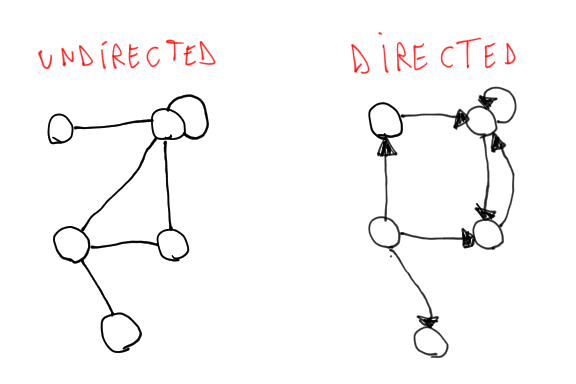
\includegraphics[height=0.6\textheight]{img/directed}
  \end{center}
\end{frame}

\begin{frame}
  \frametitle{Undirected x Directed (2)}
  \begin{block}{Why is this important?}
    \begin{itemize}
    \item In undirected graphs, the path from A to B is the same as
      the path from B to A.
    \item In directed graphs, this is not necessarily true.
    \end{itemize}
  \end{block}
  \begin{center}
    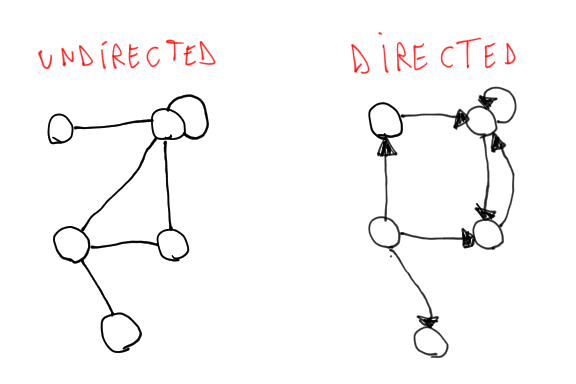
\includegraphics[height=0.6\textheight]{img/directed}
  \end{center}
\end{frame}

\begin{frame}
  \frametitle{Weighted x Unweighted (1)}
  \begin{itemize}
    \item \structure{Weighted Graphs}: Each edge in $E$ has an
      associated numerical value $w$.
    \item \structure{Unweighted Graphs}: All edges can be considered
      to have the same value (or no value).
  \end{itemize}
  \begin{center}
    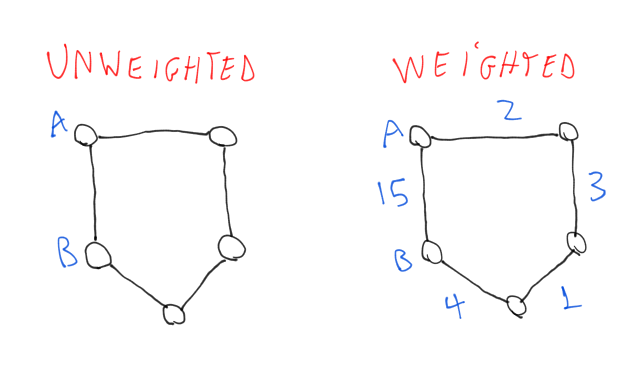
\includegraphics[height=0.6\textheight]{img/weighted}
  \end{center}
\end{frame}

\begin{frame}
  \frametitle{Weighted x Unweighted (2)}
  \begin{block}{Consequences of Weights}
    {\small
    \begin{itemize}
    \item Weights change how we define the shortest path;
    \item We can generalize unweighted graphs to graphs with weight 1;
    \item Negative weights may imply in infinite loops!
    \end{itemize}}
  \end{block}
  \begin{center}
    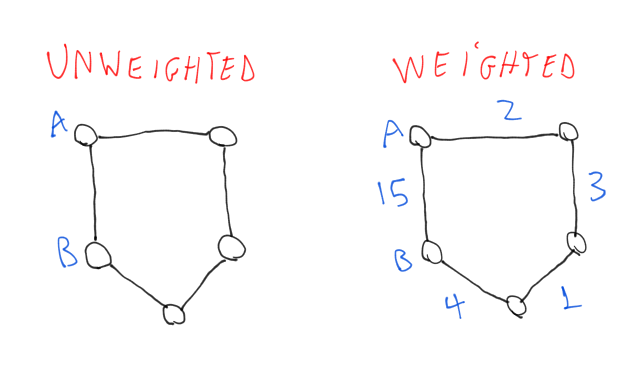
\includegraphics[height=0.6\textheight]{img/weighted}
  \end{center}
\end{frame}

\begin{frame}
  \frametitle{Cyclic x Acyclic (1)}
  \begin{itemize}
    \item \structure{Cyclic}: A subset of Vertices in the graph are
      connected as a cycle.
    \item \structure{Acyclic}: Does not contain any cycles;
  \end{itemize}
  \begin{center}
    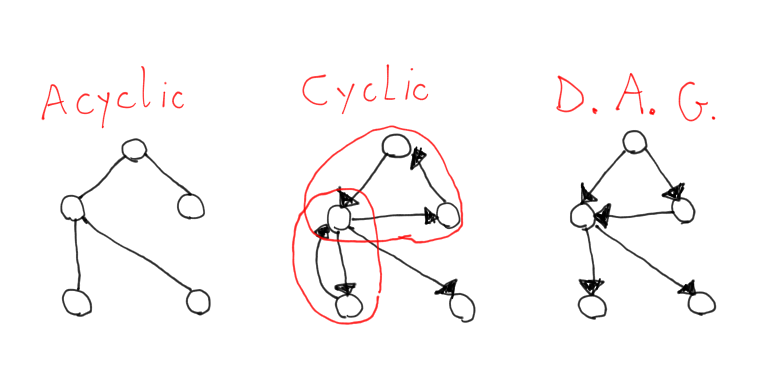
\includegraphics[height=0.6\textheight]{img/cyclic}
  \end{center}
\end{frame}

\begin{frame}
  \frametitle{Cyclic x Acyclic (2)}
  \begin{block}{Directed Acyclic Graphs}
    If a graph is both \structure{Directed} and \structure{Acyclic} at
    the same time, it can be \structure{Sorted
      Topologically}. Topological sorting is useful for a wide variety
    of algorithms.
  \end{block}
  \begin{center}
    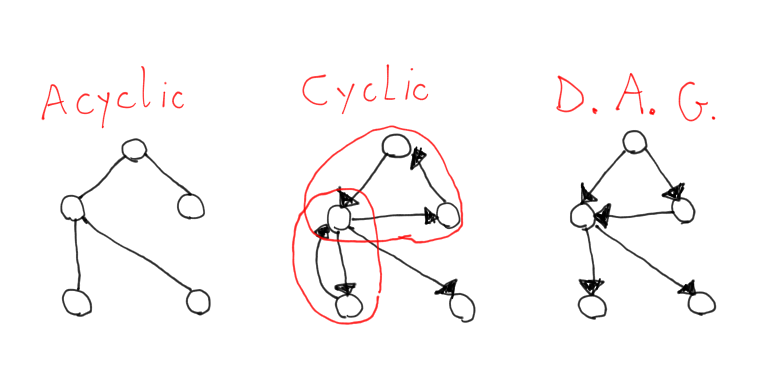
\includegraphics[height=0.6\textheight]{img/cyclic}
  \end{center}
\end{frame}

\begin{frame}
  \frametitle{Embedded x Topological (1)}
  \begin{itemize}
    \item \structure{Embedded Graphs}: Vertices and edges have been
      assigned some sort of coordinates;\\
      {\small \alert{(embedding may be relevant or not!)}}
    \item \structure{Topological Graphs}: They are completely defined
      by their embedding (edge weight equals vertice distance, etc);
  \end{itemize}
  \begin{center}
    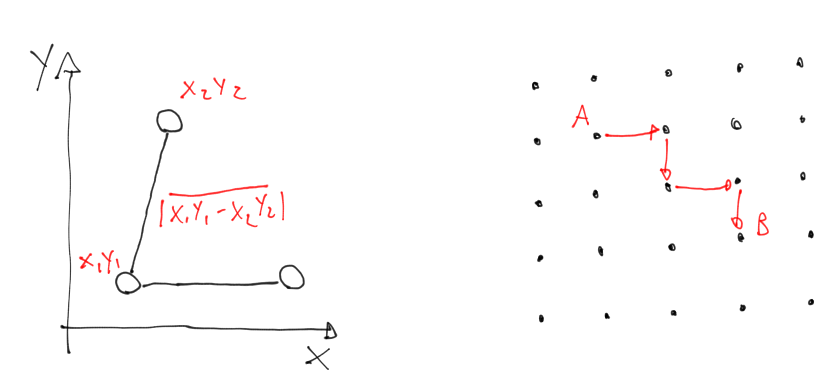
\includegraphics[height=0.5\textheight]{img/topological}
  \end{center}
\end{frame}

\begin{frame}
  \frametitle{Embedded x Topological (2)}
  \begin{block}{}
    The idea of topological graphs is to help visualize or organize
    things that are not naturally seen as graphs. For example, maps
    and paths in a map.
  \end{block}
  \begin{center}
    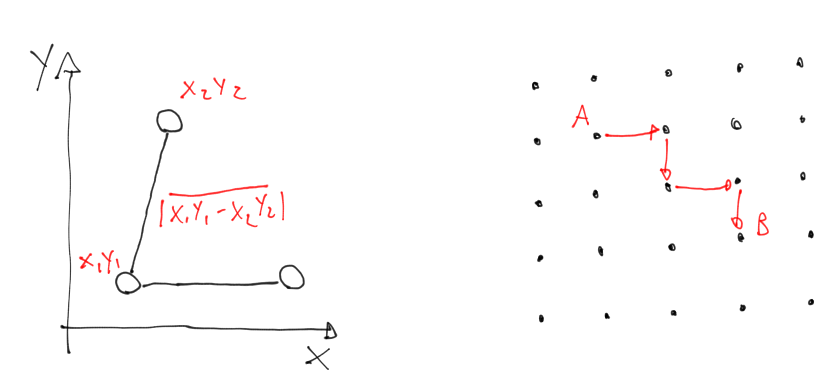
\includegraphics[height=0.5\textheight]{img/topological}
  \end{center}
\end{frame}

\begin{frame}
  \frametitle{Labelled x Unlabelled (1)}
  \begin{itemize}
  \item \structure{Labelled}: Each different vertex is assigned an unique name;
  \item \structure{Unlabelled} graphs don't have such assignments.
  \end{itemize}
  \begin{center}
    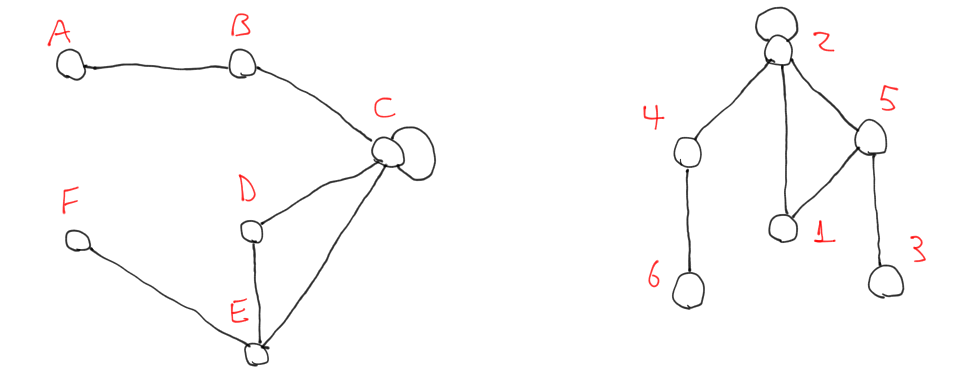
\includegraphics[height=0.45\textheight]{labelled}
  \end{center}
\end{frame}

\begin{frame}
  \frametitle{Labelled x Unlabelled (2)}
  \begin{block}{Isomorphism}
  \begin{itemize}
  \item In ``real world'' graphs (maps, processes), there is a natural labelling;
  \item Two graphs with the same structure but different labelling are
    called \structure{Isomorphic}
  \item Detecting isomorphic graphs is an important problem;
  \end{itemize}
  \end{block}
  \begin{center}
    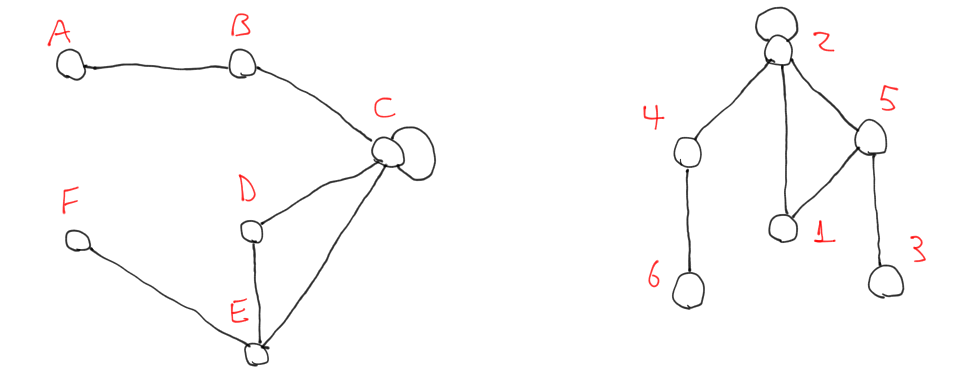
\includegraphics[height=0.45\textheight]{labelled}
  \end{center}
\end{frame}

\begin{frame}
  \frametitle{Others}
  \begin{itemize}
  \item \structure{Self Loop}: A graph with an edge $(x,x)$, involving only one vertex;
  \item \structure{Multi Edge}: The edge $(x,y)$ happens more than once on the graph;
  \item \structure{Implicit}: The graph is built as the algorithm
    progresses, it is not completely defined at the beginning.
  \end{itemize}
   \begin{center}
    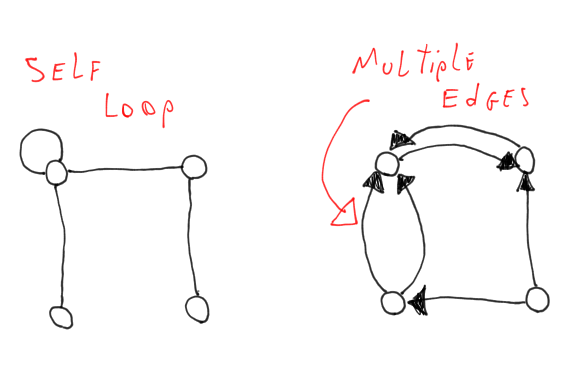
\includegraphics[height=0.45\textheight]{nonnormal}
  \end{center}
\end{frame}

\section{Structure}
\subsection{Data Structures}
\begin{frame}
  \frametitle{Quiz!}
  \begin{block}{How can we represent graphs?}
    \begin{itemize}
    \item The characteristics we presented influence in the
      representation?
    \item Is there a representation which is good for one type of
      graph, but not another?
    \end{itemize}
  \end{block}
\end{frame}

\begin{frame}
  \frametitle{Representing Graphs}
  \begin{block}{Adjacency Matrix}
      An $n \times n$ matrix where M[i,j] says whether (i,j) is an
      edge of G or not. Fast access to edges, but has some problems
      on sparse Graphs.
  \end{block}
  \begin{block}{Adjacency List in Lists}
    Array of Vertices, with linked lists of neighbors.
  \end{block}
\end{frame}

\begin{frame}[fragile,singleslide]
  \frametitle{Representing Graphs}
  \begin{block}{Adjacency List in Matrices}
    Simple to program:
    \begin{itemize}
    \item A degree array that lists the number of out-edges connected to each vertex;
    \item An edge matrix listing the adjacent vertices to each vertex.
    \end{itemize}
  \end{block}
  \medskip
  {\smaller
\begin{verbatim}
#define MAXV = 100     // maximum number of Vertices
#define MAXDEGREE = 50 // maximum vertex outdegree

typedef struct{
   int edges[MAXV+1][MAXDEGREE];
   int degree[MAXV+1];
   int nvertices;
   int nedges;
} graph;
\end{verbatim}
  } 
\end{frame}

\begin{frame}[fragile,singleslide]
  \frametitle{Representing Graphs}
  \begin{block}{Adjacency List in Matrices}
    Simple to program:
    \begin{itemize}
    \item A degree array that lists the number of out-edges connected to each vertex;
    \item An edge matrix listing the adjacent vertices to each vertex.
    \end{itemize}
  \end{block}
  \medskip
  {\smaller
\begin{verbatim}
insert_edge(graph *g, int x, int y, bool directed)
{
  g->edges[x][g->degree[x]] = y;
  g->degree[x]++
  if (directed == FALSE)
    insert_edge(g,y,x,TRUE)
  else
    g->nedges++;
}
\end{verbatim}
  } 
\end{frame}

\section{Graph search}
\subsection{Graph Traversal}
\begin{frame}
  \frametitle{Graph Traversal}
  
  \begin{block}{BFS vs DFS}
    \begin{itemize}
    \item \structure{Breadth First Search: } Order of nodes is not
      important, but we want to find the shortest paths.
    \item \structure{Depth First Search: } Easier to find cycles in
      the graph.
    \item When is each of these better?
    \end{itemize}
  \end{block}
\end{frame}

\begin{frame}[singleframe,fragile]
  \frametitle{Breadth First Search Algorithm}
  \begin{center}
    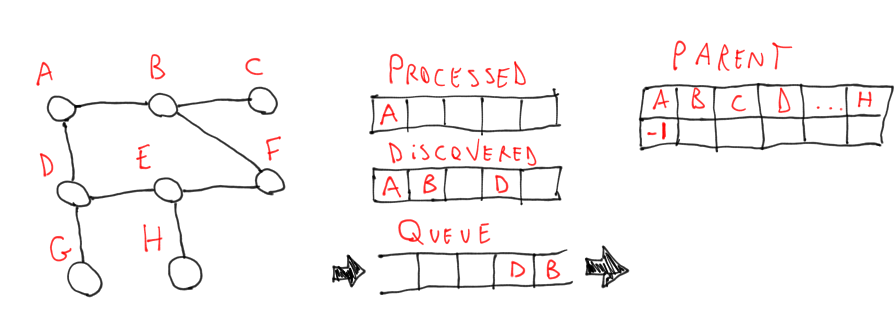
\includegraphics[height=0.4\textheight]{bfs}
  \end{center}
  \begin{block}{}
    {\small
\begin{verbatim}
Put "Start" vertex on the "queue" and "discovered";
While queue is not empty:
  v = queue.pop, put v on "processed";
  for each edge in "v", get "k" neighbor to "v":
    if k is not in "discovered":
      put k on the "queue" and "discovered";
      parent of k is v;
\end{verbatim}
    }
  \end{block}
\end{frame}

\begin{frame}
  \frametitle{BFS}
  \begin{center}
    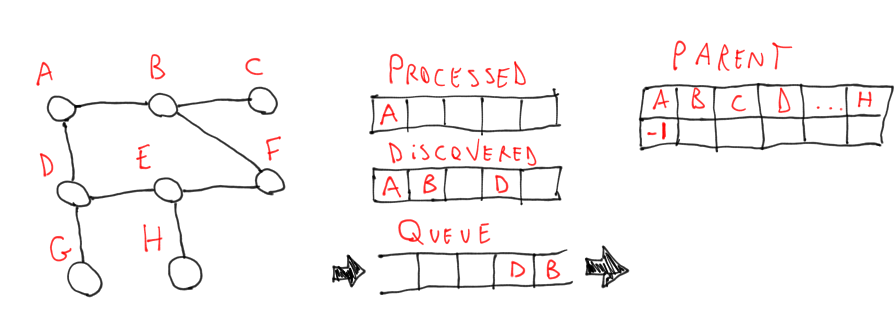
\includegraphics[height=0.4\textheight]{bfs}
  \end{center}
  \begin{block}{Finding Paths}
    \begin{itemize}
    \item By following the ``parent'' array, we can construct the
      smallest path from any node to the root of the BFS.
    \end{itemize}
  \end{block}
\end{frame}

\begin{frame}
  \frametitle{Depth First Search}
  \begin{center}
    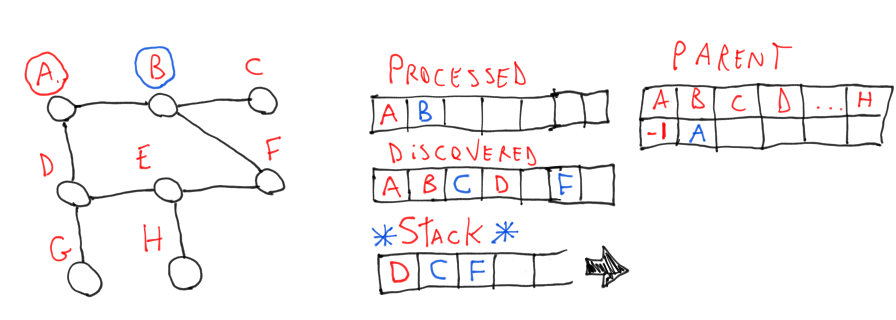
\includegraphics[height=0.4\textheight]{dfs}
  \end{center}
  \begin{block}{}
    \begin{itemize}
      \item Implementation: Stack instead of Queue
      \item Detecting Cycles: Finding a ``visited'' node while
        processing a new edge.
    \end{itemize}    
  \end{block}
\end{frame}

\subsection{Simple uses}
\begin{frame}
  \frametitle{Connected Components}
  \begin{center}
    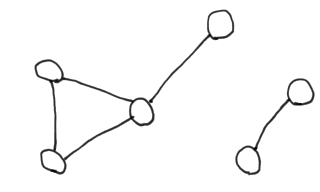
\includegraphics[height=0.35\textheight]{connected}
  \end{center}
  \begin{block}{}
    \begin{itemize}
    \item Connected Components are parts of a graph where there is a
      path between every vertice of the graph.
    \item Can be used for detecting invalid positions (in a decision
      tree graph).
    \item Can be found by DFS or BFS - any nodes not visited are not
      connected.
    \end{itemize}
  \end{block}
\end{frame}


%% REQUIRES A DIRECTED ACYCLIC GRAPH!
\begin{frame}[fragile,singleframe]
  \frametitle{Topological Sorting}
  \begin{block}{}
    \begin{itemize}
    \item Requires a Directed Acyclic Graph;
    \item Can speed up path searches by determining nodes
      ``unrelated'' to the search;
    \end{itemize}
  \end{block}
  \begin{center}
    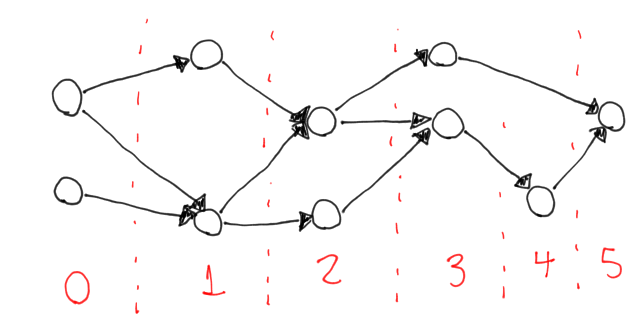
\includegraphics[width=0.55\textwidth]{topological2}
  \end{center}
\end{frame}

\begin{frame}[fragile,singleframe]
  \frametitle{Topological Sorting}
  \begin{block}{Topological Sorting Algorithm}
\begin{verbatim}
DAG topsort:
  i = 0
  while there are vertices:
    select all vertices with in-degree 0;
    give them rank "i"; i++;
    remove these vertices and their edges;
\end{verbatim}
  \end{block}
  \begin{center}
    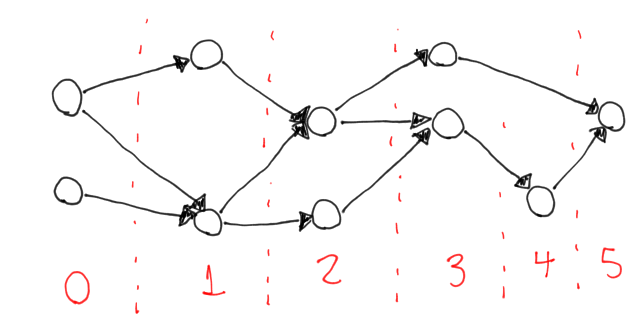
\includegraphics[width=0.55\textwidth]{topological2}
  \end{center}
\end{frame}

\section{Problems}
\subsection{Problems}
\begin{frame}
  \frametitle{This Week's Problems}
  \begin{itemize}
  \item Bicoloring
  \item Tourist Guide
  \item Slash Maze
  \item From Dusk until Dawn
  \end{itemize}
\end{frame}
\end{document}
